\documentclass[a4paper]{article}

\usepackage[english]{babel}
\usepackage[utf8]{inputenc}
\usepackage{amsmath}
\usepackage{graphicx}
\usepackage[colorinlistoftodos]{todonotes}



\author{Dylan Esguerra}

\date{September 2, 2022}

\begin{document}
\maketitle



\section{Testing text}

Professor Cook claimed that the ability to think logically and draw conclusions logically is one reason why he is good at math. Also, the fact that he is able to look for patterns and the next step in problems help him as a mathematician.

\section{Testing Math}
\label{sec:examples}


$\frac{1}{\sqrt{2\pi}}\exp{\frac{(x-\mu)^2}{\sigma^2}}$

\section{Testing picture}

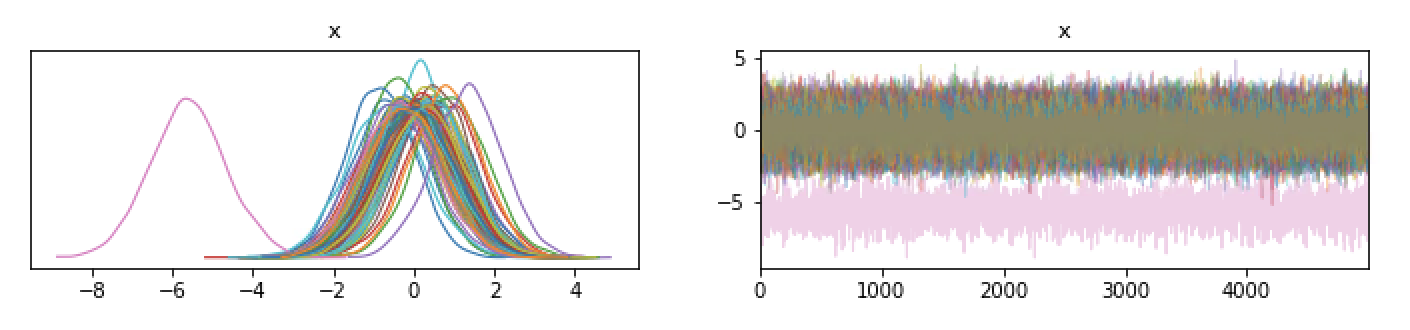
\includegraphics[scale=0.5]{trace_test.png}

\end{document}